\chapter{Le CAR-T: Nuovi approcci terapeutici al linfoma non-Hodgkin}

La terapia cellulare con CAR-T (Chimeric Antigen Receptor) è una forma di terapia genica, impiegata per forme 
refrattarie e recidivanti, i cui risultati più importanti si hanno per la leucemia linfoblastica acuta e per il 
linfoma non-Hodgkin (LNH). Sono in corso ricerche che consentano l’impiego di tale metodica anche per altre neoplasie 
ematologiche, nonché per i tumori solidi\cite{reteveneta}.

\section{Introduzione alle CAR-T}

Il CAR è un recettore transmembrana chimerico, che mediante l’utilizzo di vettori retrovirali o lentivirali, 
va a sostituire il TCR del linfocita, sfruttando il processo di ingegnerizzazione. La terapia è autologa, 
ovvero usa le cellule T proprie del paziente\cite{reteveneta}.\\
L’European Medicines Agency (EMA) ha dato l’approvazione commerciale di due CAR-T di seconda generazione: 
tisagenlecleucel (tisa-cel, KymriahTM, Novartis) e axicabtagene ciloleucel (axi-cel, YescartaTM, Gilead), 
che sono anche i prodotti disponibili in Italia\cite{reteveneta}.
Nel caso del LNH, Tisagenlecleucel è indicato per i linfomi diffusi a grandi cellule B (DLBCL) recidivanti o 
refrattari dopo due linee di chemioterapia sistemica. Axicabtageneciloleucel è stato approvato per linfomi 
diffusi a grandi cellule B (DLBCL) e linfoma a grandi cellule B primitivo del mediastino, 
refrattari o recidivanti, dopo due linee di chemioterapia sistemica\cite{EMATOCART}.\\
La FDA (Food and Drugs Administration) ha invece approvato sei farmaci CAR-T (Figura \ref{fig:FIGURE_3.8}), come 
riportato dal National Cancer Institute\cite{NIHCART}.

\begin{figure}[H]
    \begin{center}
    \vspace{-3mm}
    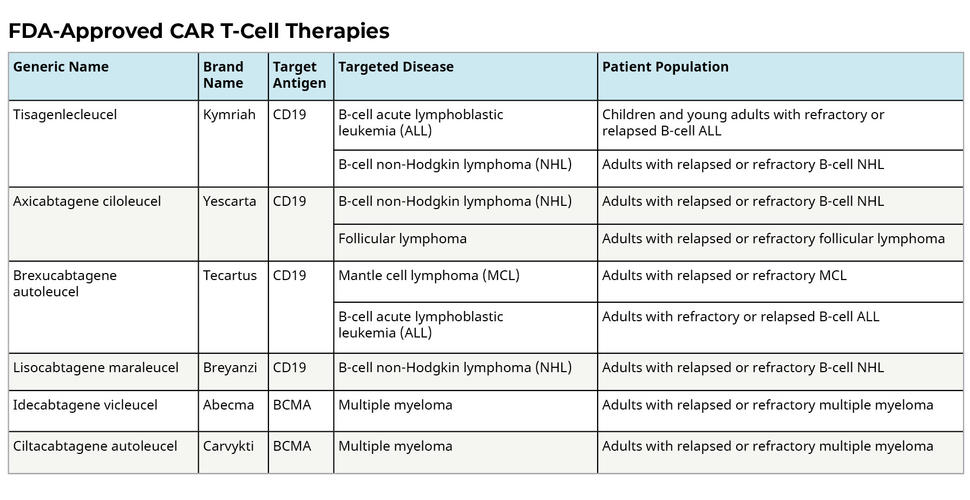
\includegraphics[width=0.9\columnwidth]{img/FDAApprovedCART.jpeg}
    \end{center}
    \caption{Farmaci CAR-T approvati dall’FDA (Food and Drugs Administration).
    \cite{NIHCART}}
    \label{fig:FIGURE_3.8}
\end{figure}

\section{Fasi del processo di costituzione delle CAR-T}

Il processo di costituzione delle CAR-T, attraversa una serie di fasi (Figura \ref{fig:FIGURE_5.2}).\\
La prima fase è la leucoaferesi, in cui viene prelevato il sangue dal 
paziente, da una vena periferica; grazie al processo di aferesi, il sangue prelevato, viene separato in 
globuli rossi, globuli bianchi, piastrine e plasma, ma solo le cellule T dei globuli bianchi saranno prelevate, 
mentre il resto del sangue viene reinfuso al paziente\cite{LLSCART}.
È una fase molto importante e delicata in quanto, una bassa resa aferetica, provoca una 
ridotta espansione delle cellule CAR-T in vitro; questo può dipendere da una bassa conta leucocitaria, 
dalla presenza di numerose cellule natural killer (NK) e blasti nel sangue periferico\cite{EMATOCART}.\\
La seconda fase del processo, prevede che le cellule T raccolte siano inviate a laboratori specializzati, per la fase 
di ingegnerizzazione genetica, secondo cui il DNA viene introdotto all’interno delle cellule, per produrre CAR, 
grazie ai quali le cellule T acquisiscono la capacità di attaccare le cellule cancerose\cite{EMATOCART}.\\
Nella terza fase, il numero di cellule raccolte viene moltiplicato in laboratorio e quando si ha il quantitativo 
necessario, vengono criopreservate e inviate al centro o all’ospedale dove il paziente le riceverà. 
Questo processo dura dalle tre alle quattro settimane\cite{LLSCART}.
Prima della somministrazione, il paziente, a partire da una settimana, fino a due giorni prima, viene sottoposto 
alla chemioterapia di linfodeplezione, che serve a ridurre le cellule T normali nel corpo, per “fare spazio” alle 
cellule CAR-T ed avere una maggiore espansione in vivo\cite{LLSCART}.
Lo schema terapeutico maggiormente utilizzato prevede la somministrazione di ciclofosfamide e fludarabina.\\
L’ultima fase è di somministrazione del farmaco, previo scongelamento, in una via endovenosa centrale, 
della durata di circa trenta minuti\cite{EMATOCART}.\\
I centri autorizzati alla somministrazione delle CAR-T sono presenti in tutta Italia, in Toscana abbiamo 
i centri di Firenze e Pisa\cite{AILCENTRI}.

\begin{figure}[H]
    \begin{center}
    \vspace{-3mm}
    \fbox{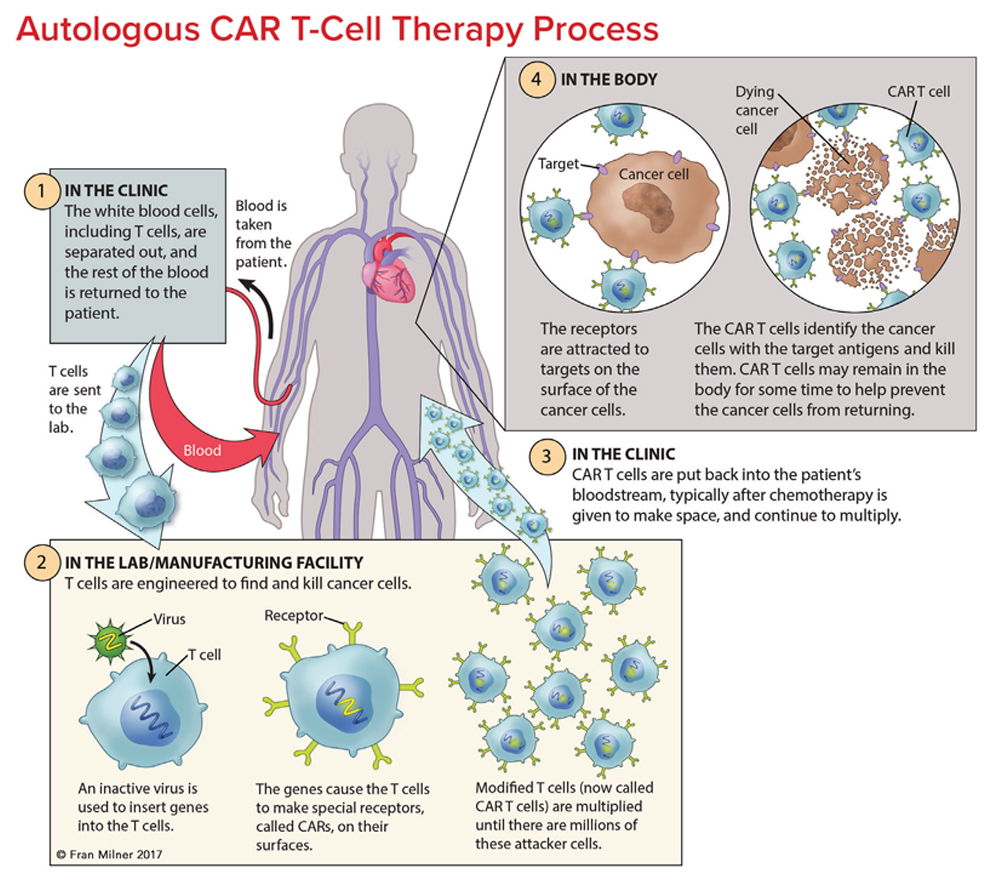
\includegraphics[width=0.7\columnwidth]{img/CART-TherapyProcess.jpeg}}
    \end{center}
    \caption{Processo di prelievo, costituzione e somministrazione delle CAR-T.
    \cite{LLSCART}}
    \label{fig:FIGURE_5.2}
\end{figure}

\section{Complicanze correlate al processo di somministrazione delle CAR-T}

Nonostante i risultati positivi dati dalla terapia delle CAR-T, che dimostrano il raggiungimento di risposte rapide e 
durature nel tempo, non mancano aspetti di tossicità acuta, che possono evolvere in situazioni di severità, se non 
anche di fatalità\cite{EMATOCART}.

\subsection{Sindrome da rilascio di citochine (CRS)}

Più frequentemente si assiste ad una sindrome da rilascio di citochine (CRS), che può manifestarsi con 
astenia, febbre, mal di testa, tachicardia, ipotensione, ipossia, arresto cardiaco, aritmia, 
encefalopatia, insufficienza renale, fino ad arrivare ad una insufficienza multiorgano.
La CRS può insorgere a partire da alcune ore, fino anche ad una settimana dalla somministrazione di CAR-T\cite{EMATOCART}.\\
Diversi sono i fattori di rischio che comportano il manifestarsi di tale sintomatologia (Figura \ref{fig:FIGURE_3.11}) 
e che influiscono anche sul suo grado di severità: l'infusione di una dose elevata di CAR-T, le caratteristiche 
del paziente, il tipo di terapia di linfodeplezione, lo stato della malattia e il burden di malattia 
(burden of disease)\cite{EMATOCART}.
La CRS può inoltre evolvere in una sindrome da attivazione macrofagica (MAS).

\begin{figure}[H]
    \begin{center}
    \vspace{-3mm}
    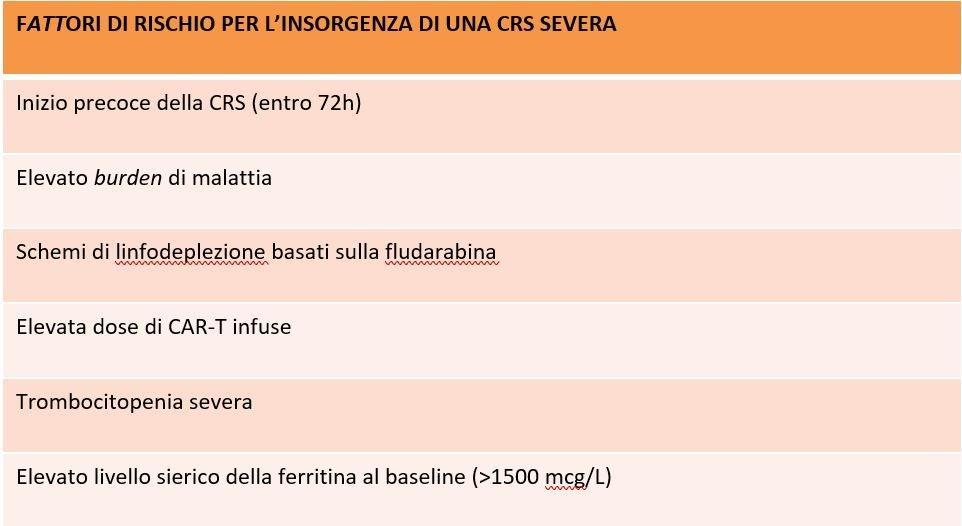
\includegraphics[width=0.7\columnwidth]{img/rischioCRS.jpeg}
    \end{center}
    \caption{Fattori di rischio per l’insorgenza di una CRS severa. 
    \cite{EMATOCART}}
    \label{fig:FIGURE_3.11}
\end{figure}

Il grado di severità con cui si sviluppa la CRS, è correlato agli elevati livelli ematici di CAR-T ed elevati livelli 
sierici di IL-6 (interleuchina-6); di conseguenza, il trattamento di prima scelta per la CRS moderata-severa, 
prevede la somministrazione di tocilizumab, un anticorpo monoclonale anti-IL-6\cite{EMATOCART}.\\
L’uso di corticosteroidi per la CRS, era precedentemente limitato, ma secondo studi più recenti il loro utilizzo 
non compromette l'attività delle CAR-T e l’outcome del paziente\cite{Cortico}.\\
Per valutare il grado di severità della CRS (Figura \ref{fig:FIGURE_5.4}), l’ASTCT (American Society for Transplantation 
and Cellular Therapy) ha prodotto delle linee guida\cite{LEE2019625}.

\begin{figure}[H]
    \begin{center}
    \vspace{-3mm}
    \includegraphics[width=0.7\columnwidth]{img/severitàCRS.jpeg}
    \end{center}
    \caption{Criteri di valutazione del grado di severità CRS.
    \cite{EMATOCART}}
    \label{fig:FIGURE_5.4}
\end{figure}

\subsection{Immune effector cell-associated neurotoxicity syndrome (ICANS)}

La neurotossicità è un effetto collaterale comune alla terapia con CAR-T. 
L’ASTCT (American Society for Transplantation and Cellular Therapy) ha definito la neurotossicità con 
l’acronimo ICANS (Immune effector cell-associated neurotoxicity syndrome). Non sono ancora del tutto chiare le 
motivazioni per cui tale sintomatologia si presenta, sono in corso studi che cercano di spiegare i meccanismi 
fisiopatologici coinvolti\cite{EMATOCART}.\\
ICANS si manifesta con afasia, disturbi dell’attenzione, difficoltà alla scrittura, confusione, disorientamento, 
agitazione, tremori e sonnolenza. In caso di ICANS severa, i sintomi che possono presentarsi sono: crisi convulsive, 
edema cerebrale, aumento della pressione intracranica, incontinenza, deficit di forza\cite{EMATOCART}.\\
È una complicanza che può presentarsi in concomitanza alla CRS, in tal caso ha una minore durata e severità; 
può insorgere anche in seguito alla CRS con maggiore durata e severità. La durata dei sintomi è variabile 
(circa 2-4 giorni o anche diverse settimane) e sono solitamente reversibili. 
Il trattamento terapeutico con tocilizumab è efficace in caso di ICANS associata a CRS, altrimenti la terapia di 
elezione è con corticosteroidi\cite{EMATOCART}.\\
L’ASTCT (American Society for Transplantation and Cellular Therapy) 
ha prodotto anche per ICANS delle linee guida per valutare il grado di severità\cite{LEE2019625}.

\begin{figure}[H]
    \begin{center}
    \vspace{-3mm}
    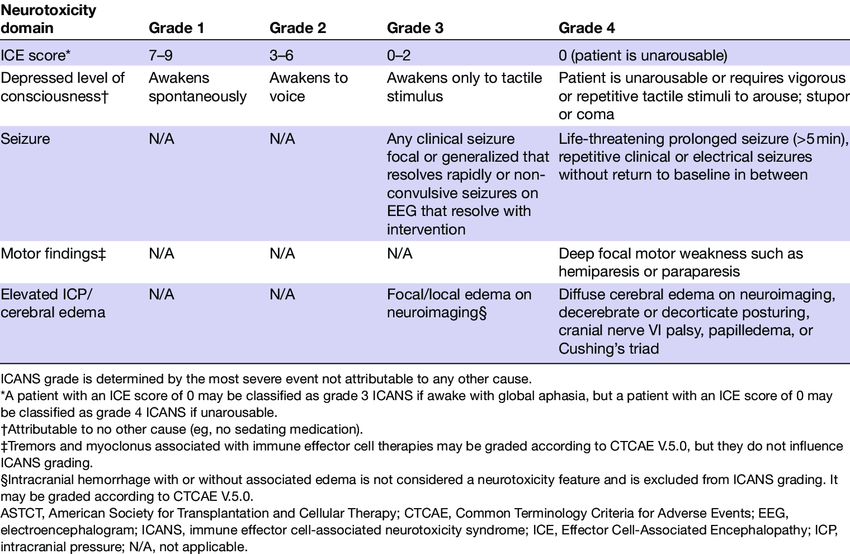
\includegraphics[width=0.8\columnwidth]{img/ICANS.png}
    \end{center}
    \caption{Parametri per la valutazione del grado di severità di ICANS.
    \cite{ICANS}}

\end{figure}

\subsection{Sindrome da Attivazione Macrofagica (MAS)}

Nella sindrome da attivazione macrofagica (MAS), si ha un’iperattività di macrofagi e linfociti, che stimolano la 
produzione di citochine pro-infiammatorie e creano degli infiltrati tissutali, con rischio di insorgenza di 
insufficienza multiorgano\cite{EMATOCART}.\\
I sintomi di CRS e MAS sono simili: febbre, sintomatologia neurologica, insufficienza multiorgano; 
gli esami ematici evidenziano livelli elevati di LDH, ferritina e citochine, mentre si
riducono i livelli di fibrinogeno\cite{EMATOCART}.
Nei pazienti in cui si sospetta una MAS, con tossicità d’organo >3, si intraprende la terapia con anticorpi monoclonali 
anti-IL-6 e corticosteroidi, in caso di non miglioramento entro 48 ore, 
si prende in considerazione la terapia con etoposide.\\
La MAS refrattaria e fulminante si presenta nell’1\% circa dei pazienti trattati con CAR-T, 
se non trattata prontamente ha un’elevata mortalità\cite{EMATOCART}.

\subsection{Altre reazioni avverse}

La tossicità autoimmune si verifica quando il linfocita CAR-T, riconosce come antigene target il CD-19, non solo nelle 
cellule cancerose, ma anche nelle cellule sane\cite{Frontiers}.
Il fenomeno è noto come “on-target-of-tissue effects”. È un effetto avverso che può risultare anche fatale.
I linfociti B sani, che presentano sulla loro superficie il target del linfocita CAR-T, vanno 
incontro ad aplasia. La ricerca, dovrebbe orientarsi a trovare una soluzione affinchè il target delle cellule CAR-T, 
siano le cellule cancerose e non quelle sane\cite{Frontiers}.\\

Una reazione anafilattica si può verificare per reazione eccessiva del sistema immunitario nei confronti del CAR, 
pertanto bisogna monitorare la comparsa di eventuali segni e sintomi come eritemi, 
sudorazione, ipotensione e distress respiratorio\cite{EMATOCART}.
Nel caso in cui si evidenzia la comparsa di tali sintomi, il trattamento viene sospeso o terminato\cite{Frontiers}.\\

Le infezioni associate alla somministrazione di CAR-T (CTI), sono piuttosto comuni.\\ Non è del tutto noto il meccanismo 
che le innesca e non c’è uno schema unico per la loro prevenzione e trattamento\cite{Frontiers}. Vi sono tuttavia una serie di fattori 
che possono indurre tali infezioni: i pazienti molto spesso sviluppano come effetto avverso alla terapia delle CAR-T 
una CRS (sindrome da rilascio di citochine), che può portare al ricovero del paziente in unità di terapia intensiva, 
dove aumenta il rischio di sviluppare infezioni nosocomiali; il trattamento con farmaci corticosteroidi per la CRS 
indebolisce il sistema immunitario, che a sua volta, risulta indebolito anche dalla riduzione di cellule B sane 
(target del CD-19 delle CAR-T); 
i pazienti che hanno un indebolimento del sistema immunitario causato dalla chemioterapia e che poi ricevono le CAR-T, 
sono ad elevato rischio di sviluppare infezioni\cite{Frontiers}.\\

La Tumor Lysis Syndrome (TLS) è una complicanza abbastanza comune, maggiormente nelle neoplasie ematologiche piuttosto 
che nelle altre\cite{Frontiers}.\\ 
Si verifica perché un elevato numero di cellule cancerose diventano necrotiche e rilasciano metaboliti e
sostanze intracellulari nel sangue e di conseguenza i reni non riescono ad eliminare completamente queste sostanze.\\ 
Segni di TLS sono iperpotassiemia, iperuricemia, iperfosfatemia e ipocalcemia, in casi gravi insufficienza renale 
acuta e aritmia\cite{Frontiers}.\\ 
Il trattamento prevede idratazione, somministrazione di diuretici e 
correzione degli squilibri idroelettrolitici; per pazienti con rischio da basso a moderato si può intraprendere la 
somministrazione di allopurinolo, in via preventiva; il rasburicase è il trattamento di elezione, come prevenzione,
sia per pazienti ad alto rischio, che per pazienti che hanno già sviluppato una TLS\cite{Frontiers}.\\

Disturbi della coagulazione a volte si presentano, tra i 6 e i 20 giorni dopo l’infusione di CAR-T. Ci sarà un  
aumento del D-dimero, il PT allungato, trombocitopenia, diminuzione del fibrinogeno. Il rischio di CID 
(coagulazione intravascolare disseminata) è maggiore in pazienti con CRS grave, 
che risulta essere direttamente proporzionale alla gravità dei disturbi della coagulazione\cite{Frontiers}.\\

La citopenia è una reazione avversa caratterizzata da neutropenia, trombocitopenia ed anemia. 
È stato dimostrato che la citopenia che insorge in seguito alla somministrazione di CAR-T, può avere una durata anche 
superiore a 30 giorni\cite{Frontiers}.
Pazienti con citopenia lieve e precoce, devono avere un supporto nutrizionale e intraprendere dei trattamenti di 
prevenzione anti-infettiva.\\ 
Per pazienti con neutropenia a lungo termine, la FDA ha approvato la somministrazione mediante iniezione di Filgrastim. 
Pazienti con anemia e trombocitopenia grave vengono sottoposti a trasfusione di sangue, globuli rossi e piastrine. 
È stato anche proposto il trapianto autologo o allogenico di cellule staminali emopoietiche, come trattamento per 
la citopenia, ma la sua efficacia non è ancora ben nota\cite{Frontiers}.

\section{L’infermiere e le CAR-T}

La diffusione, sempre più ampia, della terapia delle CAR-T, sta determinando il cambiamento del ruolo e delle 
responsabilità infermieristiche. Questa terapia, prevede per il paziente un approccio multidisciplinare, che vada a 
combinarsi con i bisogni e le difficoltà cliniche, sociali e finanziarie di cura al paziente\cite{article2}. Il ruolo svolto dagli 
infermieri è pertanto essenziale, dal punto di vista della sorveglianza clinica, coordinazione delle cure ed 
educazione al paziente, non senza difficoltà, perché queste terapie richiedono nuovi bisogni, di cui gli infermieri 
possono non avere esperienza, pertanto le strutture che eseguono queste procedure di trattamento, 
devono assicurare aggiornamento e formazione infermieristica\cite{article2}.\\

Il paziente oncoematologico che riceve il trattamento CAR-T è molto complesso, agli infermieri è richiesto 
di agire, con l’abilità di riconoscere, monitorare e classificare eventuali tossicità\cite{NURSINGCART}.\\
Il fatto che, ad oggi, le CAR-T, siano un’opzione di trattamento per stati di malattia relativamente avanzati o comunque 
per forme recidive/refrattarie che non hanno risposto ad altri trattamenti (standard o terapie sperimentali), 
genera sentimenti d’ansia, i pazienti possono soffrire di isolamento sociale, soprattutto se sono in cura in centri 
lontani dalla loro sede e di conseguenza dalle persone significative\cite{NURSINGCART}. Tutto il team multidisciplinare deve essere a 
conoscenza di questi fattori; il nursing prevede di assicurarsi che il paziente, i familiari e la figura del caregiver, 
ricevano le giuste informazioni che riguardano test, procedure, istruzioni sulla gestione dell’accesso 
venoso centrale e le potenziali complicanze che ne potrebbero derivare\cite{NURSINGCART}.\\
Bisogna sottolineare il ruolo centrale che gli infermieri hanno nell’impiego delle CAR-T, dalla preparazione del 
paziente, prelievo delle cellule del paziente stesso, infusione delle CAR-T costituite, nella post-infusione, 
ed anche nel follow-up\cite{NURSINGCART}.\\

Quando il paziente è candidato a ricevere la terapia CAR-T, l’infermiere, per garantire sicurezza al trattamento, 
deve accertarsi che abbia eseguito tutti i test necessari, per quanto riguarda la valutazione della funzionalità epatica, 
renale, cardiaca e polmonare\cite{article2}. Prima dell’infusione, effettuare i controlli necessari, per ridurre il 
rischio di complicanze che potrebbero derivare da infezioni batteriche, virali e fungine\cite{NURSINGCART}.\\
Potrebbe rendersi necessaria una "bridging chemotherapy", ovvero dei cicli di chemioterapia nel caso in cui 
la malattia sia particolarmente aggressiva da potersi espandere, se non trattata nel periodo di tempo di attesa della 
ricostituzione delle CAR-T. In tal caso, bisogna comunque considerare gli eventuali rischi associati alla chemioterapia
(Tumor Lysis Sindrome, Sindrome da Rilascio di Citochine)\cite{article3}.
Inoltre è opportuno valutare il “burden of disease” del paziente, cioè l’impatto che 
la malattia ha in termini di disabilità e mortalità.\\ 

Per la somministrazione di CAR-T, gli infermieri devono tenere conto di una serie di passaggi: identificare il paziente e 
illustrare la procedura, verificare la presenza del consenso informato firmato in cartella, controllare la correttezza 
della prescrizione, rilevare i parametri vitali, assicurando che il paziente sia apiretico ed emodinamicamente stabile, 
documentare in cartella, controllare l’accesso venoso; predisporre nelle vicinanze del paziente, il carrello delle 
emergenze, verificando che tutto il materiale sia presente e i dispositivi funzionanti\cite{NURSINGCART}. 
Somministrare eventuale pre-medicazione se prevista, iniziare l’infusione usando i set di infusione che arrivano con 
le cellule, monitorare la comparsa di eventuali reazioni correlate all’infusione. 
Paziente e caregiver devono essere informati in forma verbale e scritta, riguardo possibili reazioni avverse, 
si renderà necessario riferire eventuali sintomi e rimanere nelle vicinanze dell’ospedale per almeno 4 settimane dopo 
la terapia; assicurarsi che il paziente eviti di guidare per 8 settimane dopo l’infusione\cite{NURSINGCART}.\\

Indipendentemente dallo svolgimento del trattamento in regime ambulatoriale o di ricovero ordinario, 
il ruolo dell’infermiere durante l’infusione del prodotto resta imperativo; essi devono essere adeguatamente 
formati e pronti, riguardo la gestione di  effetti avversi che possono verificarsi durante l’infusione, 
già al momento della presa in carico del paziente\cite{article2}.\\
Il riconoscimento e la classificazione precoce, possono aiutare gli infermieri oncologici, nella selezione di interventi 
basati sulle evidenze, che possano permettere la gestione e l’annullamento di effetti collaterali potenzialmente 
minacciosi per la vita stessa del paziente. Agli infermieri, si consiglia di adottare nella pratica clinica, 
metodi di classificazione e valutazione oggettivi, come parte dell’agire quotidiano, soprattutto nei 
casi in cui si sospettano complicanze come la neurotossicità, i cui cambiamenti possono insorgere 
rapidamente nel tempo\cite{article4}.\\

Parte del management infermieristico prevede oltre alla valutazione del paziente, anche l’accertamento, da parte 
dell’infermiere, della presenza di tutti i mezzi di supporto necessari al paziente durante il trattamento. 
Ad esempio alcuni centri di cura, richiedono al paziente di restare ad una specifica distanza dal centro stesso, 
fino a 30 giorni dopo l’infusione di CAR-T, per consentire l’accesso del paziente alla struttura, in tempi ragionevoli, 
nel caso insorgessero complicanze o effetti avversi dopo la dimissione\cite{article2}.\\ 
Prima dell’approvazione del paziente per il trattamento, si effettua un consulto infermieristico in cui si accerta 
la presenza del caregiver, il cui ruolo si dimostra di cruciale importanza,
poiché le istituzioni si muovono sempre di più verso una scelta ambulatoriale per l’esecuzione di tali procedure, 
per ridurre i costi e i ricoveri in ospedale\cite{article2}. 
Questa esigenza, si traduce nel bisogno di educare il caregiver, nel riconoscimento precoce di segni e sintomi delle 
principali complicanze correlate all’infusione delle CAR-T, nonché sull’importanza di riferire eventuali potenziali 
effetti avversi al team sanitario.\\ Come riportato dall’autore, senza un caregiver adatto a rispondere ai 
bisogni del paziente in modo appropriato, il paziente potrebbe non essere un candidato ottimale 
alla terapia delle CAR-T\cite{article2}.\\

Vista la crescita nell’uso delle CAR-T, la ONS (Oncology Nursing Society), ha sviluppato una risorsa, 
proprio con lo scopo di migliorare l’apprendimento dei meccanismi correlati ai vari processi che costituiscono 
le CAR-T, gli effetti avversi potenzialmente più comuni e le considerazioni infermieristiche su come trattarli\cite{ONSCART}.

\begin{figure}[H]
    \begin{center}
    \vspace{-3mm}
    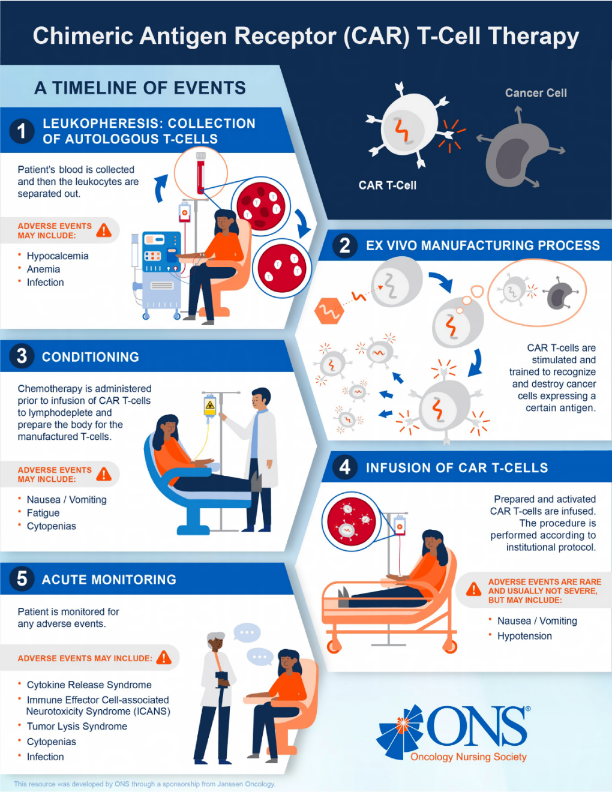
\includegraphics[width=0.9\columnwidth]{img/onsCAR-T.png}
    \end{center}
    \caption{Risorsa ONS (Oncology Nursing Society) fasi del processo CAR-T.
    \cite{ONSCART}}

\end{figure}

\begin{figure}[H]
    \begin{center}
    \vspace{-3mm}
    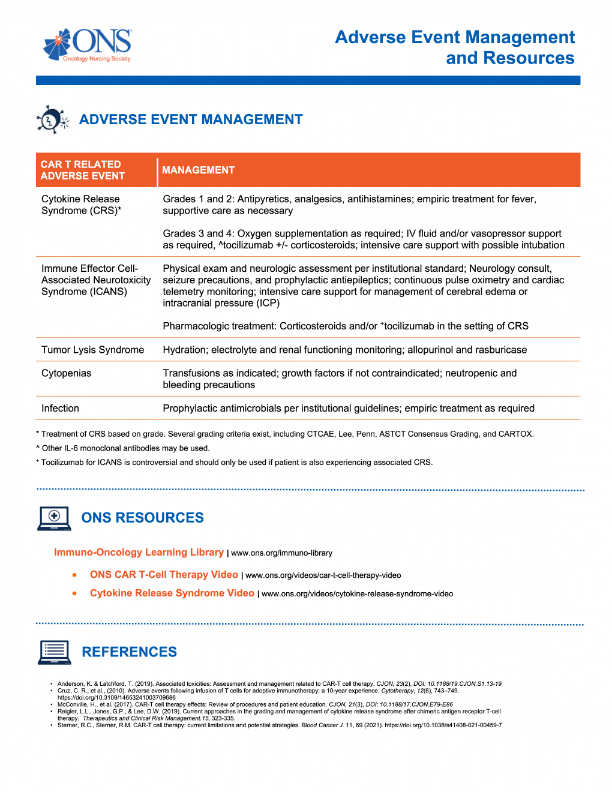
\includegraphics[width=0.9\columnwidth]{img/ONS.png}
    \end{center}
    \caption{Risorsa ONS (Oncology Nursing Society) complicanze della terapia CAR-T e loro gestione.
    \cite{ONSCART}}

\end{figure}

\section{Regime dietetico del paziente oncologico}

Il paziente ematologico, può attraversare una fase di neutropenia, immunodepressione non neutropenica oppure può essere 
sottoposto a cicli di chemioterapia non intensiva\cite{DIETA}. A ciascuna di queste fasi, corrisponde un regime dietetico.\\
La condizione di neutropenia si verifica in genere dopo circa 30 giorni dalla chemioterapia o dal trapianto di 
cellule staminali. Lo spessore della parete intestinale tende a ridursi e a fissurarsi, l’intestino perde la capacità 
di assorbire alimenti complessi e di conseguenza si presenteranno dolori addominali e diarrea, con il 
rischio che la flora batterica intestinale, entri in circolo e provochi delle infezioni sistemiche\cite{DIETA}.\\ Dal punto di vista 
igienico e nutrizionale, bisogna avere una serie di accorgimenti: prestare particolare attenzione alla 
pulizia, lavare bene le mani prima di preparare il pasto e prima di mangiare, mantenere la cucina disinfettata; si può 
effettuare il lavaggio in lavastoviglie impostando programmi ad alte temperature;
lavare gli strofinacci giornalmente; il paziente non deve condividere le proprie posate con altri; 
le confezioni di latte e le lattine devono essere pulite prima di conservarle e aprirle; 
acquistare i cibi controllando sempre la data di scadenza, le confezioni devono essere sigillate e possibilmente 
in dosi da consumare all’apertura senza conservarle nuovamente; 
la carne, il pesce e le uova devono essere consumati ben cotti; gli alimenti congelati devono essere scongelati in 
frigo o al microonde, ma non a temperatura ambiente e cucinarli prontamente; conservare gli avanzi di cibo 
in frigo in contenitori chiusi e consumarli entro 24 ore; 
non consumare cibi cotti con griglie da barbecue destinate all’esterno, a meno che 
non siano adeguatamente lavate e preriscaldate. Consultare il medico, prima di consumare erbe, spezie, vitamine, 
minerali e alcolici. Per le cene fuori al ristorante, informarsi dopo quanto tempo è possibile farlo, evitare comunque 
i pasti a buffet\cite{DIETA}.\\

Il paziente immunodepresso non neutropenico, possiede delle difese sufficienti, tuttavia bisogna seguire degli 
accorgimenti ed evitare determinati cibi\cite{DIETA}. La dieta deve prevedere 
un adeguato apporto di proteine, pochi grassi, frutta e verdura cruda possono essere consumate, ma accuratamente 
lavate. Evitare il latte crudo non pastorizzato, la ricotta e gli yogurt, evitare formaggi stagionati come 
brie, gorgonzola e ricotta salata; carne e pesce devono essere ben cotti, evitare gli affumicati e i 
marinati (pancetta, speck, salsiccia, pesci e frutti di mare), nonché birra non pastorizzata, lievito crudo e
non bere l’acqua del rubinetto\cite{DIETA}.\\
La dieta ipercalorica può essere richiesta dal medico per far recuperare il peso perso dal paziente nel corso delle 
terapie precedenti. Si può aumentare la quota calorica consumando pasta, riso, cereali, pane e patate; 
nonchè pesce, carne e uova, verdure cotte e insalate, legumi, latte e derivati, frutta e introdurre le fonti di grassi, 
attraverso olio d’oliva, avocado e burri di frutta secca\cite{DIETA}. 
Seguire una dieta sana e bilanciata, limitando il consumo di alimenti con grassi 
saturi, zuccheri aggiunti e limitare il consumo di sale. Per gli alcolici, se concessi, 
limitarsi ad un drink per la donna, due per l’uomo\cite{LLSNUTRITION}.\\
Gli effetti collaterali correlati al trattamento, come perdita dell’appetito, mucositi, nausea, alterazioni del 
gusto, rendono difficoltosa l’assunzione del cibo, potrebbe essere utile fare delle passeggiate prima dei pasti per 
stimolare l’appetito, fare pasti piccoli e frequenti, assumere cibi che piacciono, non mangiare da soli ma in compagnia, di 
amici o familiari\cite{LLSNUTRITION}.

\section{Il dolore nel paziente oncologico}

Il dolore è considerato il quinto parametro vitale ed è uno dei sintomi che più preoccupa il paziente, 
in quanto impatta negativamente sulla qualità di vita.\\ La gestione del dolore, 
è una delle dimensioni di cura più importanti, il ruolo degli infermieri è fondamentale, 
dal punto di vista sia della valutazione, sia per quanto riguarda il trattamento farmacologico e non farmacologico. 
Risulta essenziale impostare un’adeguata terapia, poiché il dolore non trattato può 
influenzare gli esiti della malattia ed evolvere a dolore cronico persistente\cite{BOOK3}.\\
Nell'attività quotidiana, l'infermiere dedica buona parte dell'assistenza alla relazione con il paziente instaurando
un rapporto empatico; questo elemento è imprescindibile per capire nel miglior modo possibile, l'entità del
dolore del paziente. Sebbe­ne per la misurazione vengano utilizzati metodi validati, senza la collabo­razione del 
paziente non è possibile stabilire la giusta sede, il tipo di dolo­re e il livello di intensità, 
poiché il dolore resta un sintomo soggettivo\cite{BOOK3}.\\
Un aspetto fondamentale è la valutazione iniziale, ma è altret­tanto indispensabile la rivalutazione frequente del paziente, 
in quanto permette di determinare se gli interventi adottati sono stati effi­caci nel ridurre la 
sintomatologia\cite{BOOK3}.\\

Il dolore è un’esperienza multidimensionale, che coinvolge la sfera biologica, psicologica e sociale, ed è 
influenzata da fattori ambientali; può essere di tipo acuto, cronico o persistente e i pazienti possono 
provare tutti questi tipi di dolore insieme, per cui diventa difficile comprendere l’esperienza provata\cite{PAINONS}.\\ 
Il dolore del paziente oncologico, dipende dal tipo di neoplasia, dalle terapie antineoplastiche e
dalla presenza di comorbilità. Bisogna valutare il dolore per quanto riguarda: 
localizzazione (i pazienti possono riferire di avere dolore anche in più di un punto, talvolta chiedere di 
localizzarlo può aiutare a capirne la causa), tipo di dolore (neuropatico, somatico o viscerale), intensità 
(da valutare utilizzando le scale di valutazione del dolore) da quanto tempo è insorto, 
se è continuo o intermittente, qual è il piano terapeutico attuale per il controllo del dolore e la risposta 
del paziente ad esso; considerare che il dolore di tipo refrattario, nel 10-20\% dei pazienti, 
non risponde all’analgesia standard\cite{CANCERPAINONS}.\\
Le scale di valutazione del dolore sono unidimensionali (Figura \ref{fig:FIGURE_5.8}) e multidimensionali.
Le prime sono orientate a misurare l'intensità del dolore, come 
la scala VAS (Scala Visuale Analogica), 
la scala di valutazione numerica (NRS),
la scala di valutazione verbale (VRS) e la Facies Pain Scale (FPS), utilizzata
per la valutazione del dolore nel bambino;
le seconde, come il Brief Pain Inventory (BPI), McGill Pain Questionnaire (MPQ) 
e PAINAID, descrivono il dolore non solo valutando l'intensità, ma anche altri aspetti, 
come l'interferenza dello stesso nelle attività di vita quotidiana.\\ Le scale unidimensionali sono di più 
facile compilazione, quelle multidimensionali forniscono un maggior numero di informazioni, ma per via della loro 
complessità, non sono facilmente applicabili nella pratica clinica\cite{BOOK3}.

\begin{figure}[H]
    \begin{subfigure}[b]{0.5\textwidth}
            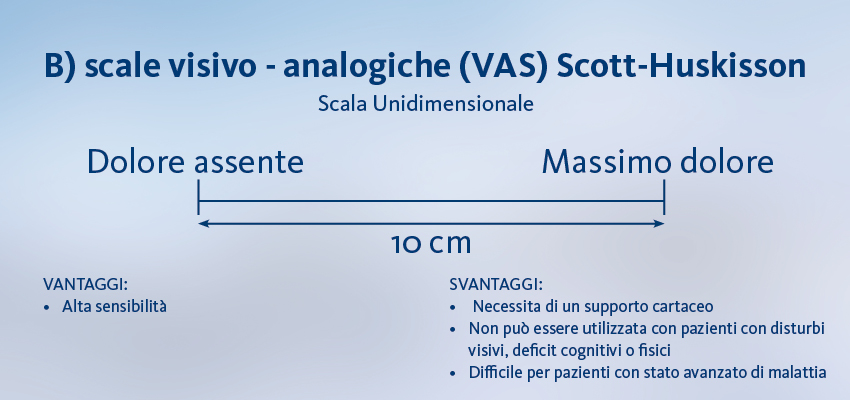
\includegraphics[width=\linewidth]{img/VAS.jpeg}
            
           
    \end{subfigure}
    \begin{subfigure}[b]{0.5\textwidth}
        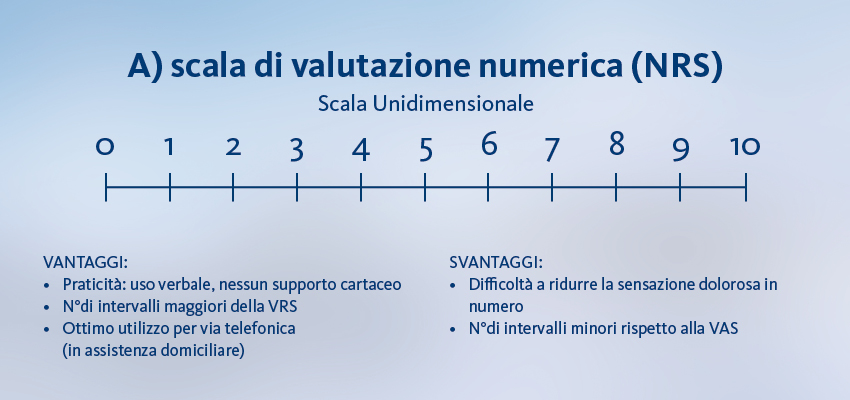
\includegraphics[width=\linewidth]{img/NUMERICA.jpeg}
        
        
\end{subfigure}
    \begin{subfigure}[b]{0.5\textwidth}
        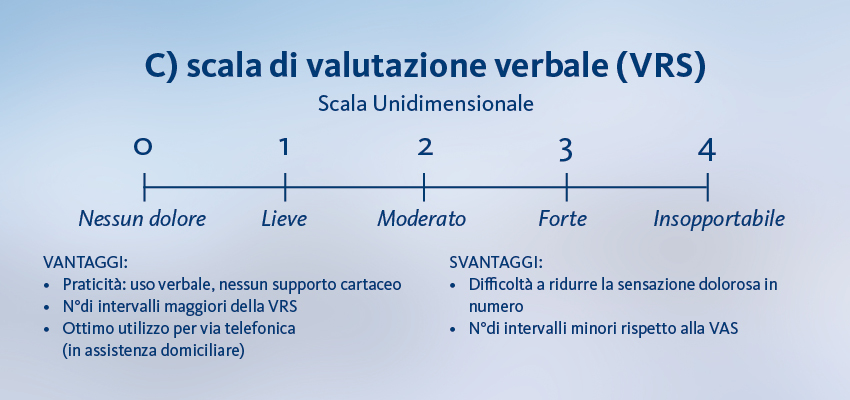
\includegraphics[width=\linewidth]{img/VERBALE.jpeg}
    
    
\end{subfigure}
    \begin{subfigure}[b]{0.5\textwidth}
     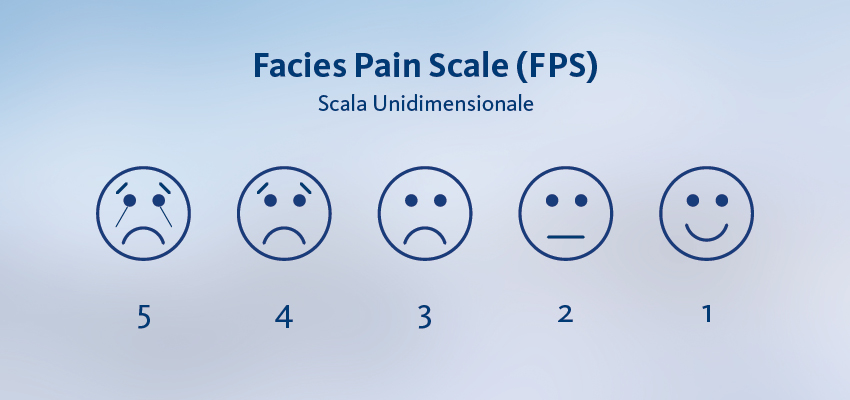
\includegraphics[width=\linewidth]{img/FACCINE.jpeg}
    
    
\end{subfigure}
    \caption{Scale unidimensionali di valutazione del dolore. \cite{SCALEDOLORE}}
    \label{fig:FIGURE_5.8}
    
\end{figure}

Da uno studio condotto, gli infermieri, non hanno abbastanza conoscenze riguardo la corretta gestione del dolore
(sono stati riportati risultati medio-bassi)\cite{PAIN}; essi pertanto devono essere adeguatamente formati, 
dal momento che all’interno del team di assistenza, sono le figure più importanti coinvolte con i pazienti 
oncologici.\\
Secondo le stime  della WHO (World Health Organisation), più del 90\% del dolore oncologico può essere 
controllato con interventi di routine. Nonostante siano molti gli interventi da poter attuare seguendo le evidenze, 
i pazienti continuano a soffrire, perché le pratiche non vengono applicate quotidianamente\cite{PAINONS}.\\
Gli infermieri devono mettere in atti una valutazione completa, sistematica ed accurata del dolore usando 
strumenti appropriati. Uno di questi è il NOC (Nursing Outcomes Classification), che si basa sulle diagnosi infermieristiche\cite{painNOC}. 
La selezione degli esiti dei NOC, per la valutazione di pazienti in cure palliative ospedaliere, si è dimostrata 
importante per guidare la pratica clinica, considerando la specificità dell’assistenza in questo settore\cite{painNOC}.
Questo aspetto deve essere incentivato all’approfondimento, visti i riscontri positivi della ricerca, ma anche la limitata 
produzione scientifica.\\
Tra le terapie non farmacologiche, è stato dimostrato che l’utilizzo del massaggio terapeutico, ha effetti positivi sul 
controllo del dolore in pazienti oncologici sottoposti a cure palliative, migliora la circolazione sanguigna e linfatica, 
riduce l’edema e l’infiammazione, rilassa i muscoli, aumenta i livelli di 
serotonina e dopamina, nonché il numero di linfociti\cite{tpnonfarmacologiche}.\\

Le problematiche di dipendenza/abuso di oppioidi, possono interferire con l’ottimale gestione del dolore oncologico. 
È una questione che rappresenta un dilemma per medici e infermieri, che spesso, per paura di instaurare problematiche di 
dipendenza, evitano la prescrizione di tali farmaci; in questo modo però, il dolore non viene gestito e 
i pazienti continuano a soffrire\cite{PAINONS}.\\ 
Secondo la ONS (Oncology Nursing Society), la responsabilità degli infermieri e dei medici, nei confronti 
del paziente e dei familiari, è di agire applicando le EBP (evidence based practice)\cite{PAINONS}.\\
Vi sono evidenze che dimostrano che è possibile somministrare oppioidi per il controllo del dolore nei pazienti con SUDs 
(substance use disorders), fondamentale è la prevenzione delle ricadute\cite{CANCERPAINONS}. 
Riconoscere le ricadute può essere difficile, 
questi pazienti tendono a nasconderlo, per cui bisogna programmare un percorso di detossificazione graduale, 
da non vedere come un fallimento, ma come parte del processo di guarigione\cite{CANCERPAINONS}.\\
Nonostante le numerose discussioni, i farmaci analgesici e gli oppioidi in particolare, restano fondamentali per 
la gestione del dolore oncologico moderato-severo. Probabile preoccupazione per i pazienti con dolore oncologico, 
è lo sviluppo di tolleranza agli analgesici, cioè se si assumono tali farmaci ogni volta che c’è bisogno, poi questi 
non saranno efficaci quando il dolore sarà più intenso. I regimi analgesici dovrebbero pertanto essere 
determinati in collaborazione con il paziente per garantire un uso sicuro e ridurre al minimo i risultati negativi\cite{analgesici}. 

\section{La comunicazione tra infermiere e paziente}

L’infermiere è il professionista sanitario che stabilisce una relazione di aiuto costante e prolungata con 
il paziente oncologico e i suoi familiari. Fornisce supporto psicologico ed emotivo, promuove il ruolo del caregiver e del 
nucleo familiare, aiuta il paziente nel processo di accettazione dei cambiamenti 
che intervengono nella sua vita, a causa sia della malattia, sia del presidio venoso, che ha lo scopo di facilitare il 
programma di cura, ma con possibili complicanze\cite{COMUNICAZIONE}.\\
L’infermiere deve essere consapevole del suo ruolo professionale, deve agire con competenza e se non 
sufficientemente preparato è obbligato a formarsi ed aggiornarsi.\\
Il processo di assistenza infermieristica comprende l'identificazione dei problemi infermieristici, del paziente e 
della famiglia, la pianificazione di interventi, l’implementazione di un piano di assistenza sulla base degli 
obiettivi prefissati, la valutazione dei risultati ottenuti\cite{COMUNICAZIONE}.\\
Il supporto al paziente viene dato mediante l’educazione del paziente stesso, circa lo stile di vita, la dieta, la 
gestione delle complicanze, la descrizione di procedure diagnostico-terapeutiche e il controllo dei sintomi, ma bisogna 
anche riuscire a sviluppare nel paziente una capacità di autocura e autogestione della malattia, orientandolo 
verso l’autonomia\cite{NURSE24}.\\
L’infermiere oltre a sapere e saper fare, deve saper essere, ovvero possedere quelle capacità comunicative e 
relazionali, insieme ad empatia e umanità, che sono proprie della sua figura; deve promuovere la 
consapevolezza della malattia e la conoscenza del percorso clinico-assistenziale, sostenendo la persona nella 
scelta del trattamento più adatto\cite{COMUNICAZIONE}.\\
Il bisogno emotivo del paziente, si traduce in un bisogno di informazioni, di rassicurazione, vicinanza emotiva, 
empatia, pertanto l’infermiere deve essere preparato ad accogliere la sofferenza del paziente e dei suoi familiari\cite{NURSE24}.\\
I pazienti molto spesso avvertono un profondo senso di solitudine, causato dall’impossibilità di comunicare con i 
loro cari e le persone significative, non riescono ad occupare le giornate in modo attivo, questo 
perchè talvolta sono sottoposti a ricoveri in regime di isolamento, oppure in unità operative ad accesso controllato 
(come la terapia intensiva), hanno bisogno di assistenza per le attività pratiche e questo può provocare 
nel paziente profondo disagio\cite{NURSE24}.\\
Si parla di comunicazione terapeutica quando si entra in sintonia con l’altro ed egli riesce a chiedere aiuto e a 
sentirsi ascoltato, compreso, accettato e non giudicato.

